\chapter{LLMを用いた話しことば検出 \label{c7}}

本章では,LLMを用いた話しことばを検出させる実験について述べる.LLMが持つ話しことばの知識を本システムの話しことばルールを比較し,ChatGPTがもつ話しことばの認識について調査した。

\subsubsection{使用したデータ}
本実験では,2019年度に本学で開講された,2年次が履修する「アルゴリズムとプログラミング」の講義内で提出されたレポートから16件を抽出し,その本文を用いた.後述の各検証では一律でこのデータを用いている.

\subsubsection{検証方法}
検証は,プロンプトに話しことばの検出をせる内容の指示を入力し,得られた出力結果を話しことばチェッカーに通す.このときの出力結果は「話しことばとされたもの」と呼ぶことにし,話しことばチェッカーで検出された話しことばの種類数を精度の指標とし,LLMの話しことばの認識について調査した.

本章の検証では,ChatGPT APIからGPT-4を利用している.表\ref{table-parameter}にAPI使用時のパラメータ設定を示す.

検証時に,話しことばチェッカーで検出した話しことばおよびグレーゾーンの種類を表\ref{result-checker-detect}に示す.

\begin{table}[H]
\caption{API使用時のパラメータ設定}
\label{table-parameter}
\begin{tabular}{|l|l|r|}
\hline
\multicolumn{1}{|c|}{パラメータ名称} & \multicolumn{1}{c|}{説明} & \multicolumn{1}{c|}{値} \\ \hline
Temperature& \begin{tabular}[c]{@{}l@{}}生成する文章のランダム度合を表す.\\ 値が低いほど毎回の出力で同じ生成結果を得やすい.\end{tabular} & 0 \\ \hline
Max\ tokens& 生成する文章の長さを指定する. & 1000 \\ \hline
Frequency penalty & 同じトークンの出やすさを制御する. & 0.4 \\ \hline
\end{tabular}
\end{table}

% 使用箇所: c7
\begin{table}[H]
\centering
\caption{話しことばチェッカーでの検出結果}
\label{result-checker-detect}
\begin{tabular}{|l|r|}
\hline
話しことばの種類 & 20 \\ \hline
グレーゾーン & 2 \\ \hline
\end{tabular}
\end{table}

\section{Few-shot Prompting を用いた話しことば検出 \label{c7s1}}
主観・客観の分類では,文章と分類結果を1組にして,プロンプトに与える例示に組み込んだ.本検証でも同様に,例文とその中に含まれている話しことばを1つの例としてプロンプトに組み込み,話しことば検出を行った.

\begin{table}[H]
\centering
\caption{Few-shot Promptingを用いた話しことば検出のためのプロンプト}
\small % \footnotesize
\begin{tabular}{|l|}
\hline
\multicolumn{1}{|c|}{プロンプト} \\ \hline
\begin{tabular}[c]{@{}l@{}} 
\#\#\# 役割 \#\#\#\\
あなた(GPT)を,「大学初年次における日本語文章教育のエキスパート」\\とします。\\
\\
\#\#\# 指示 \#\#\#\\
与えられた文章から、話しことばである表現を抽出してください。\\
ここでの話しことばの定義は「学術表現として使用することが適切\\ではない表現」です。\\
話しことばを抽出したとき、以下の情報を出力してください。\\
1. 抽出した話しことば\\
\\
\#\#\# 例 \#\#\#\\
Q. 以下の文章から、話しことばである表現を抽出してください。\\
日本人はお米を食べるのが当たり前のくせにパンばかり食べる。\\この件の対応策の策定は政府がやらなければならないとされており、\\政府は検討して要望を提出すると述べている。\\
A. 抽出した話し言葉は以下の通りです。\\
   - 抽出した話しことば1 : 当たり前\\
   - 抽出した話しことば2 : くせに\\
   - 抽出した話しことば3 : やらなければならない\\
   - 抽出した話しことば4 : 検討して\\
\\
Q. 以下の文章から、話しことばである表現を抽出してください。\\
高台の家はあやうく浸水被害を免れた。日頃から防災意識を持つ\\ことの必要性を痛いほど実感した。\\
A. 抽出した話し言葉は以下の通りです。\\
   - 抽出した話しことば1 : あやうく\\
   - 抽出した話しことば2 : くせに\\
\\
(中略)\\
\\
Q. 以下の文章から、話しことばである表現を抽出してください。\\
少子化問題の根本的な解決策はわからない。\\
A. 抽出した話し言葉は以下の通りです。\\
   - 抽出した話しことば1 : わからない
\\
Q. 以下の文章から、話しことばである表現を抽出してください。\\
自ら走ることもあるので\\
A. 抽出した話し言葉は以下の通りです。\\
   - 抽出した話しことば1 : ので\\
\\
\#\#\# 実践 \#\#\# \\
Q. 以下の文章から、話しことばである表現を抽出してください。\\
(レポート本文)
\end{tabular}   \\ \hline
\end{tabular}
\label{prompt-detectspoken-few10}
\end{table}

プロンプトは,LLMが内容を正しく読み取れることを考慮し,LLMに役割を与える「役割」,取り組んでほしいタスクを示した「指示」,「話しことばの具体例」,「書きことばリスト」,「学生のレポート本文(検出をさせる文章)」のように構成した.

本検証では,与える例を0, 2, 5, 10, 40件のときに分けて検証を行った.

\subsection{結果}
LLMの検出結果を表\ref{result-detectspoken-few10}に示す.すべての場合で120種類以上の表現を話しことばとして検出したが,実際に話しことばであったものは,多くても8種類であり,ほとんどすべてが話しことばではない表現であった.

\begin{table}[H]
\caption{Few-shot Promptingを用いたときの検出結果}
\label{result-detectspoken-few10}
\centering
\begin{tabular}{|l|r|r|r|r|r|}
\hline
 & \multicolumn{1}{c|}{zero-shot} & \multicolumn{1}{c|}{\begin{tabular}[c]{@{}c@{}}few-shot\\ 例2件\end{tabular}} & \multicolumn{1}{c|}{\begin{tabular}[c]{@{}c@{}}few-shot\\ 例5件\end{tabular}} & \multicolumn{1}{c|}{\begin{tabular}[c]{@{}c@{}}few-shot(10)\\ 例10件\end{tabular}} & \begin{tabular}[c]{@{}r@{}}話しことば\\ チェッカー\end{tabular} \\ \hline
\begin{tabular}[c]{@{}l@{}}話しことばとして\\ 検出されたもの\\ (単位: 種類)\end{tabular} & 120 & 125 & 135 & 125 & - \\ \hline
\begin{tabular}[c]{@{}l@{}}チェッカーで検出\\ した話しことば\end{tabular} & 6 & 8 & 5 & 5 & 20 \\ \hline
グレーゾーン & 2 & 2 & 2 & 2 & 2 \\ \hline
\begin{tabular}[c]{@{}l@{}}実際は話しことば\\ ではなかったもの\end{tabular} & 106 & 114 & 130 & 118 & - \\ \hline
\end{tabular}
\end{table}

\subsection{考察}
話しことばの検出に焦点を当てていたが,話しことばと対になる存在である書きことばについて言及していないことや,どのようなものが書きことばであるかを理解できていないことが考えられる.これを踏まえ,次節では,書きことばの具体例を新たにプロンプトに組み込んで検証を行った.

\section{書きことばリストを用いた話しことば検出 \label{c7s2}}
明らかに書きことばであると考えられる表現を列挙し,これらの表現を検出しないように指示を加えたプロンプトを用いた検証を行った.
書きことばリストには,誤検出で特に多かった表現を選択している.

\begin{table}[H]
	\centering
        \caption{書きことばリスト}
 	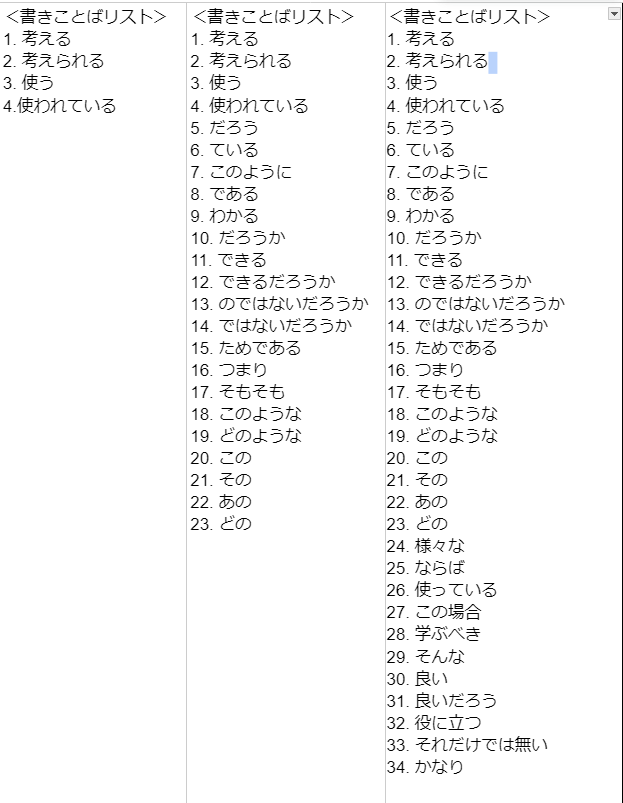
\includegraphics[width=80mm]{image/image-klistTable.png}
	\label{klistTable}
\end{table}

本検証では,\ref{c7s1}節の例40件を与えたときと与えなかったときで比較している.

\subsection{結果}
本検証の結果を表\ref{result-klist-few40},表\ref{result-klist-few0}に示す.例示を入れている方では検出数は70種類以上あるが,実際に話しことばであるものは
\begin{table}[H]
\caption{書きことばリスト組込み時の話しことば検出結果(例あり)}
\label{result-klist-few40}
\centering
\begin{tabular}{|l|r|r|r|}
\hline
\begin{tabular}[c]{@{}l@{}}書きことばリスト\\ の件数\end{tabular} & 4 & 23 & 34 \\ \hline
\begin{tabular}[c]{@{}l@{}}話しことばとして\\ 検出されたもの\\ (単位: 種類)\end{tabular} & 96 & 77 & 90 \\ \hline
\begin{tabular}[c]{@{}l@{}}チェッカーで検出した\\ 話しことば\end{tabular} & 13 & 11 & 12 \\ \hline
グレーゾーン & 2 & 1 & 2 \\ \hline
\begin{tabular}[c]{@{}l@{}}話しことばでは\\ なかったもの\end{tabular} & 81 & 65 & 76 \\ \hline
\end{tabular}
\end{table}
\begin{table}[H]
\caption{書きことばリスト組込み時の話しことば検出結果(例なし)}
\label{result-klist-few0}
\centering
\begin{tabular}{|l|r|r|r|}
\hline
\begin{tabular}[c]{@{}l@{}}書きことばリスト\\ の件数\end{tabular} & 4 & 23 & 34 \\ \hline
\begin{tabular}[c]{@{}l@{}}話しことばとして\\ 検出されたもの\\ (単位: 種類)\end{tabular} & 64 & 58 & 49 \\ \hline
\begin{tabular}[c]{@{}l@{}}チェッカーで検出した\\ 話しことば\end{tabular} & 11 & 10 & 10 \\ \hline
グレーゾーン & 2 & 1 & 2 \\ \hline
\begin{tabular}[c]{@{}l@{}}話しことばでは\\ なかったもの\end{tabular} & 51 & 47 & 37 \\ \hline
\end{tabular}
\end{table}

\subsection{考察}
例を与えたときの方が例を与えなかったときよりも誤検出が多く,検出できた話しことばの種類の数に大きな変化が無く,相対的に検出の精度が低くなることがわかった.このことから,\ref{c7s1}節の方式での例示では話しことば検出の効果が低いことが考えられる.

\section{話しことば・書きことばの定義を変更したときの話しことば検出 \label{c7s3}}
プロンプトには話しことばの定義を記述していたが,LLMが生成した話しことばの定義を利用することで誤検出が減らせると仮定し,LLMに話しことばの定義を生成させ,一部編集を加えたものをプロンプトに組み込み,これを用いて話しことば検出を行った.

\begin{table}[H]
\centering
\caption{プロンプト中の話しことば・書きことばの定義の変更点}
\label{spoken-written-def}
\begin{tabular}{ll}
 & 定義の内容 \\
\begin{tabular}[c]{@{}l@{}}変更前の話しことば・\\ 書きことばの定義\end{tabular} & \begin{tabular}[c]{@{}l@{}}話しことば: 学術表現として使用することが\\ 適切ではない表現\end{tabular} \\
\begin{tabular}[c]{@{}l@{}}変更後の話しことば・\\ 書きことばの定義\end{tabular} & \begin{tabular}[c]{@{}l@{}}書きことば: 公的文書や学術論文、技術文書\\ などで一般的に使用されるフォーマルな表現\\ \\ 話しことば: 日常生活で使う文章や敬語の文章\\ で使用されるインフォーマルな表現\end{tabular}
\end{tabular}
\end{table}

\subsection{結果}

\begin{table}[H]
\centering
\caption{話しことば検出結果}
\label{result-expert}
\begin{tabular}{|l|r|}
\hline
話しことばとして検出されたもの(単位: 種類) & 60 \\ \hline
チェッカーで検出した話しことば & 15 \\ \hline
グレーゾーン & 2 \\ \hline
話しことばではなかったもの & 43 \\ \hline
\end{tabular}
\end{table} % 移行忘れず

\begin{table}[H]
	\centering
        \caption{書きことばリストに載っている表現の出現頻度}
 	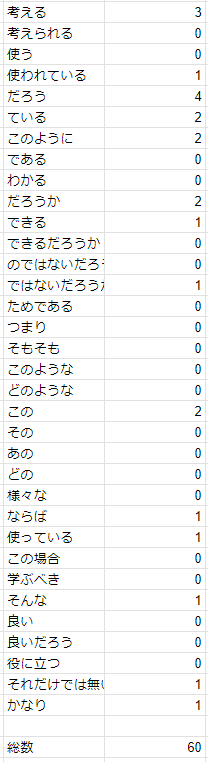
\includegraphics[width=50mm]{image/kenshutu-ichiran-old.png}
	\label{kenshutu-ichiran-old}
\end{table}

\subsection{考察}
書きことばリストを導入したときよりも誤検出が増えた.これは,定義を変更したことにより,定義に沿った検出結果を生成したことが考えられる.

\section{指示を2段階に分けたときの話しことば検出 \label{c7s4}}
書きことばリストにあげられている表現が依然として多いため,得られた出力結果を用いて,書きことばリストに載っている表現を除去するように再度指示を与えた.

\begin{table}[H]
\centering
\caption{話しことば検出のためのプロンプト(後半部)}
\small % \footnotesize
\begin{tabular}{|l|}
\hline
\multicolumn{1}{|c|}{プロンプト} \\ \hline
\begin{tabular}[c]{@{}l@{}} 
\#\#\# 指示 \#\#\# \\
以下の<書きことばリスト>の1から34までの表現は書きことばとします。<書きことばリスト>の言葉が\#\#\# 表現リスト \#\#\#に含まれている場合、\#\#\# 表現リスト \#\#\#から除外して出力してください。
<書きことばリスト>
1. 考える
2. 考えられる
3. 使う
4. 使われている
5. だろう
6. ている
7. このように
8. である
9. わかる
10. だろうか
11. できる
12. できるだろうか
13. のではないだろうか
14. ではないだろうか
15. ためである
16. つまり
17. そもそも
18. このような
19. どのような
20. この
21. その
22. あの
23. どの
24. 様々な
25. ならば
26. 使っている
27. この場合
28. 学ぶべき
29. そんな
30. 良い
31. 良いだろう
32. 役に立つ
33. それだけでは無い
34. かなり

\#\#\# 表現リスト \#\#\# \\
(1度目の出力で得られた「話しことばとされたもの」)
\end{tabular}   \\ \hline

\end{tabular}
\label{prompt-sdetectspoken-klist}
\end{table} % なぜこのプロンプトにしたか書こう

% プロンプトの内容は,表\ref{prompt-detectspoken-api},表\ref{prompt-sdetectspoken-klist}の書きことばリストの部分を抜き取り,\ref{c7s1}節の結果から書きことばリストに当てはまる表現を除去する内容である.

\subsection{結果}
上記のプロンプトで得られた話しことば検出結果を表\ref{kenshutu-ichiran-imp}に示す.

\begin{table}[H]
\centering
\caption{話しことば検出結果}
\label{result-checker-klist2times}
\begin{tabular}{|l|r|}
\hline
話しことばとして検出されたもの(単位: 種類) & 46 \\ \hline
チェッカーで検出した話しことば & 13 \\ \hline
グレーゾーン & 2 \\ \hline
話しことばではなかったもの & 31 \\ \hline
\end{tabular}
\end{table} % 移行忘れず

\begin{table}[H]
	\centering
        \caption{書きことばリストに載っている表現の出現頻度}
 	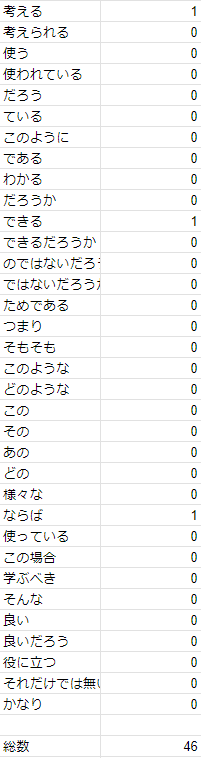
\includegraphics[width=50mm]{image/kenshutu-ichiran-imp.png}
	\label{kenshutu-ichiran-imp}
\end{table}

\subsection{考察}
指示を2段階に分けることにより,書きことばの減少が確認できた.一度の処理では,ChatGPTは最初に書かれた指示を優先して行い,その後の指示を読み取ることが難しいと考えられる.

\section{専門家による判定}
\ref{c7s4}節の結果のうち,話しことばチェッカーで話しことばではないと判定された表現を専門家に判定してもらった.総数は重複を含め21件である.判定項目は(1)話しことばである,(2)グレーゾーン(主観的または客観的),(3)グレーゾーン(判定不能),(4)話しことばではないの4項目である.判定結果を表\ref{bunruikekka}に示す.左列が該当の表現,中央はその表現が含まれている文章,右列は専門家による判定である.

\begin{table}[H]
	\centering
        \caption{専門家の判定結果}
 	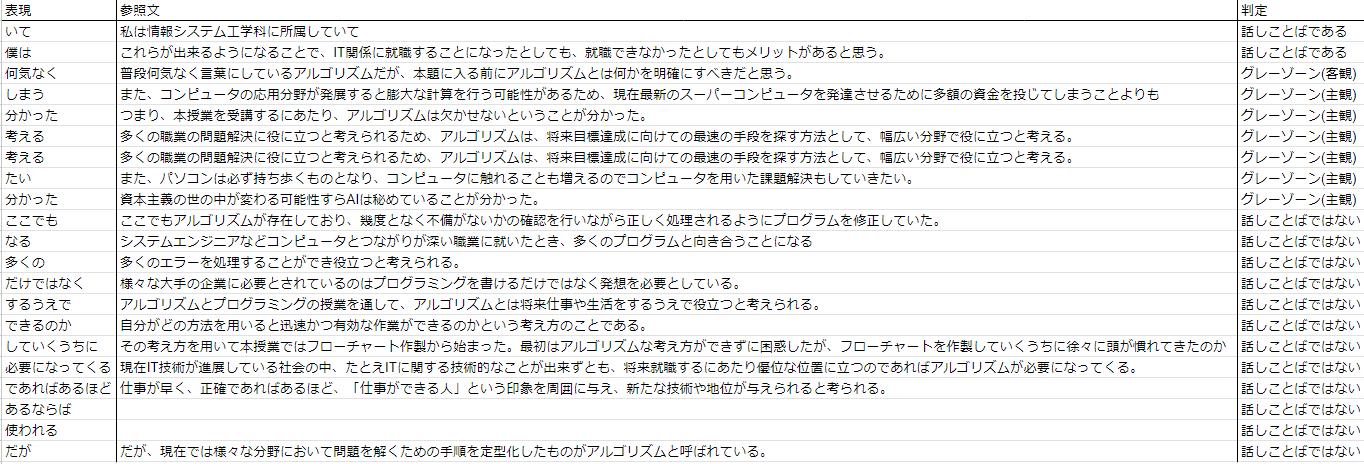
\includegraphics[width=150mm]{image/result-bunruikekka.png}
	\label{bunruikekka}
\end{table}

判定の結果は,話しことばであるものが2件,グレーゾーンであるものが計7件,話しことばではなかったものが12件となり,新規の話しことばが見つかったが,半数は話しことばではない結果となった.

\subsection{考察}
\ref{c7s3}節で使用した定義によって検出された表現のほとんどが話しことばと認められなかった.これについて,LLMはプロンプトに入力した話しことばの定義「日常生活で使う文章や敬語の文章で使用されるインフォーマルな表現」に沿った話しことば検出を行っているが,この定義が本研究チームの話し言葉の定義と異なり,専門家の想定している話しことばと異なる表現を話しことばとして検出したためと考えられる.また,書きことばの定義「公的文書や学術論文、技術文書などで一般的に使用されるフォーマルな表現」としており,書きことばの基準を高く認識している可能性がある.